\begin{surferPage}[Kummer'in Dörtgili]{Kummer'in Dörtgili}
    Eduard Kummer 1875 yılında derecesi $d$ olan bir yüzey üstünde en fazla tekillik
sayısının ($\mu(d)$ diye gösteriyoruz) kaç olabileceğini özel olarak derecesi $4$ olan yüzeyler 
(yani \emph{dörtgiller}) için soran ilk kişi oldu.

Kummer $\mu(4)=16$ olduğunu gösterdi. Bunun ardından $16$ tekilliği olan dörtgilleri ayrıntısıyla çalıştı.     \[\bigl(x^2+y^2+z^2-\mu^2\bigr)^2 - \lambda
    \,y_0\,y_1\,y_2\,y_3,\]
yüzeyler ailesi, o tür yüzeyleri içeren kayda değer güzellikte bir ailedir.
Burada  $\mu$  bağımsız bir parametre ve 
    $\lambda = \frac{3\mu^2-1}{3-\mu^2}$; 
$y_i$'ler bir düzgün dörtyüzlünün yüzlerini oluşturan düzlem ifadeleri:
 {\small
    $y_0=1-z-\sqrt{2}x$, \  
    $y_1=1-z+\sqrt{2}x$, \ 
    $y_2=1+z+\sqrt{2}y$, \ 
    $y_3=1+z-\sqrt{2}y$.}
Böylece inşa edilen yüzey dörtyüzlü simetrisine sahip oluyor.
Bu ailenin tüm üyeleri tam $16$ gerçel tekilliğe sahip değil, ama çoğu öyle:
  \begin{center}
    \vspace*{-0.2cm}\hspace*{-0.2cm}
    \begin{tabular}{@{}c@{\,}c@{\,}c@{\,}c@{\,}c@{}}
      \begin{tabular}{@{}c@{}}
        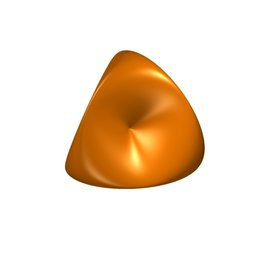
\includegraphics[height=1.4cm]{./../../common/images/kummer_0}
      \end{tabular}
      &
      \begin{tabular}{@{}c@{}}
        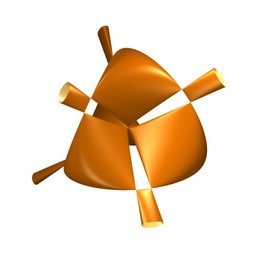
\includegraphics[height=1.4cm]{./../../common/images/kummer_1}
      \end{tabular}
      &
      \begin{tabular}{@{}c@{}}
        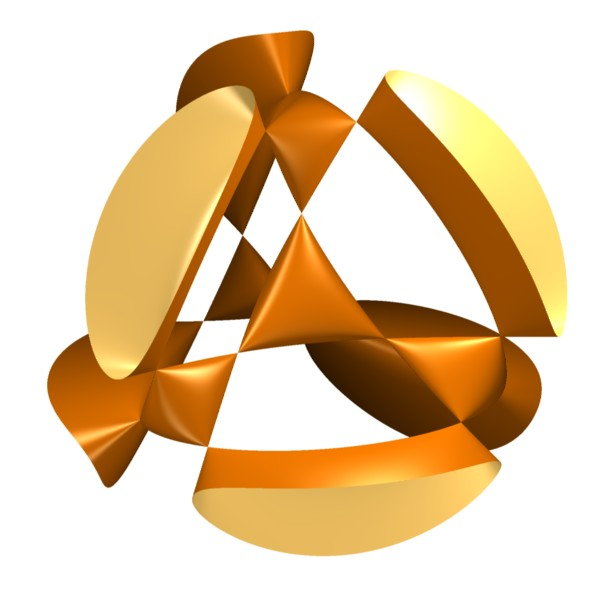
\includegraphics[height=1.4cm]{./../../common/images/kummer_2}
      \end{tabular}
      &
      \begin{tabular}{@{}c@{}}
        
\includegraphics[height=1.4cm]{./../../common/images/kummer_3}
      \end{tabular}
    \end{tabular}
  \end{center}
  \vspace{-0.2cm}  
Parametrelerin bazı özel değerleri için tekilliklerden birkaçı üstüste gelebiliyor.
\end{surferPage}
